\documentclass[conference]{IEEEtran}
\IEEEoverridecommandlockouts
% The preceding line is only needed to identify funding in the first footnote. If that is unneeded, please comment it out.
\usepackage{cite}
\usepackage{amsmath,amssymb,amsfonts}
\usepackage{algorithmic}
\usepackage{graphicx}
\usepackage{textcomp}
\usepackage{xcolor}
\def\BibTeX{{\rm B\kern-.05em{\sc i\kern-.025em b}\kern-.08em
    T\kern-.1667em\lower.7ex\hbox{E}\kern-.125emX}}

\begin{titlepage}
   \begin{center}
    
        \vspace*{1cm}

        \textbf{\large PROJECT SYNOPSIS \\ on}
            
        \vspace{1.5cm}
        
        \textbf{\LARGE Automatic IDS Signature Generation using Honeypot}\\
        
        \vspace*{0.5cm}
        to be submitted by
        \vspace{1.5cm}

        \textbf{Mehtab Zafar, Ashish Joshi, Nitish Sharma, Mohammad Anas}\\
        \vspace{0.5cm}
        1703010100, 1703010037, 1703010119, 1703010102\\
        \vspace{1.5cm}
        for the award of the degree of\\
        \vspace{1.5cm}
        \textbf{BACHELOR OF TECHNOLOGY}\\
        in\\
        {\LARGE Computer Science and Engineering}
        \vspace{2.5cm}
        
        
\includegraphics{college}
        
        \vspace{1.5cm}
        {\LARGE INDERPRASTHA ENGINEERING COLLEGE, GHAZIABAD}\\
        {\normalsize SESSION - 2020-21}
                
   \end{center}
\end{titlepage}

\begin{document}
\maketitle
\newpage
\begin{abstract}

Main aim of this project would be to integrate honeypot and IDS, which can then be used to automatically generate and activate the snort rule based on the data collected by the honeypot. The crucial part of securing the computer networks is to make them more secure. Technologies like Intrusion Detection System (IDS) are usually the software used for such a process. IDS provides security by detecting an attackers activity and analyzing their behaviour and keeps tracks of those by storing a unique hash called signature. We will implement a Honeypot which when integrated with Snort IDS would improve the capabilities of detecting the intrusion on the main server. \\
We present an architecture that uses basic principles of computer networking, virtualization, and Cyber Security and integrate these with intrusion detection systems, in order to protect networks characterized by a constantly changing underlying infrastructure and physical topology. Our goal is to define a process and a novel architecture that minimizes the security risk in networks. Above architecture involves analyzing the behavioral signature of the user logging into the system and capturing new attacks.
\end{abstract}

\begin{IEEEkeywords}
Virtualization, Intrusion detection system, cloud networks, honeypots, Snort
\end{IEEEkeywords}

\section{Introduction}

The considerable increase in usage of the internet has led to an increase in the number of cyber crimes (e.g., identity theft, data theft). So there was a need for something that monitors network traffic for suspicious activities. For this very purpose various Intrusion Detection Systems (IDS) were designed.  IDS is a software application that scans a network or a system for harmful activity / security breaches and sends a report to the backend server. Many IDS were designed for this in the past which increases the target system visibility and detects the direct attacks. These IDS are: (1) Host Intrusion Detection System (HIDS) - higher visibility at lower attack resistance, (2) Network Intrusion Detection System (NIDS)- higher attack resistance at a cost of visibility, but the drawback to these signature-based systems is their inability to detect new or previously unknown attacks. If no signature exists to match an attack type, the new attack will go undetected, this is the reason we are using VIDS which provides resistance to direct attacks at good visibility.\\

The main functions of IDS are: 

\begin{itemize}
\item Monitoring and analyzing both user and system activities.
\item Analyzing system configurations and vulnerabilities. 
\item Assessing system and file integrity. 
\item Ability to acknowledge the existence of patterns of typical attacks.
\item Analysis of anomalous activity patterns.
\item Tracking user policy violations.
\end{itemize}
\\
All the concept revolves around VMM (Virtual Machine Monitor) which is another layer inspecting hardware and the software components. This ability to interpose at the hardware interface also allows us to perform interactions between the hardware and the host software, allowing us to perform both intrusion detection and hardware access control. Virtual Machines can run different operating systems and consider that they have complete control over hardware dedicated to them. The suggested virtual intrusion detection system will use the concept of honeypots to detect intrusions and assert logs which can be further used by admin of the network to prepare for new invasions and methodology used by hackers.\\
Snort network-based intrusion detection system (IDS) has the ability to perform real-time traffic analysis and packet logging on the incoming traffic. Snort performs protocol analysis and content matching \cite{b1} for detecting various kinds of intrusion toward a system. It can also be used to detect probes or attacks, operating system fingerprinting attempts, stealth port scans. SNORT IDS provide three modes (network intrusion detection, packet sniffer, packet logger) of operations \cite{b2}. In network intrusion mode, IDS will monitor network traffic and analyze it against a rule set defined by the user. In the sniffer mode, the program will read network packets and display them on the console. And in the packet logger mode it logs all the IP packets.\\
A honeypot is a security mechanism that is built to deflect the attackers.A Honeypot is attached to the network and is set up to be a decoy of the original server. It lures the attackers, and as they try to gain unauthorized access to the server it records their activities. Since they are great at documenting exploits. Attackers tending to compromise a honeypot, its attack-related information, such as the IP address, will be collected and saved as logs. These logs provide valuable information and analysis of these attacking techniques, allowing system administrators to trace back and prepare for new invasions and methodology used by hackers.\\
Honeypots are basically of two kind (1) High-Interaction Honeypot (2) Low Interaction honeypots. In our project we'll be developing a low-interaction honeypot since it will be simulating only 1 or 2 services.
The primary objective is to reduce hardware usage by performing routing and switching virtually and maintaining a network with minimal usage of hardware.

\section{Brief Literature Survey}
In order to develop a Honeypot which would be best suited to integrate with an IDS a thorough study on the Honeypot development process is needed. The honeynet project \cite{b3} and the book \cite{b4} provides guidelines on how to implement honeypots. There have been a few attempts to design systems with self generating signatures based on logging information. One of the first attempts is the Honeycomb \cite{b5}. An evaluation of Honeycomb performed in \cite{b6}, states that Honeycomb produces too many signatures on traffic which is not malicious. This leads to a lot of false alarm.

In this project we plan to use SNORT, an intrusion prevention system which drop packets based on SNORT rules. In order to find out how to convert the data captured by honeypot into new signatures for SNORT, a study on how a SNORT \cite{b7} signature is built would be required.

Automatic SNORT signature generation based on honeypot activities has been developed at various universities and research labs. Department of Informatics & Electrical, Del Institute of Technology \cite{b8} developed a web based honeypot to generate rules and signatures that could be used by SNORT IDS for detecting intrusion via HTTP traffic.

Norwegian Information Security Laboratory - NISlabs \cite{b9} did a research to find out how much user interaction would be needed to be able to generate new signature rules for new attacks. They also researched about which honeypot would be best suited for obtaining the useful data.

\section{Scope of the project}

\subsection{System Requirements}
\begin{itemize}
    
\item A Virtual Private Server (VPS) having a LINUX Operating System support with minimum of 1GB RAM and 25GB Solid-State Drive (SSD).
\item The Ubuntu 20.04 TLS Operating System will be running on the VPS, which will be running the Honeypot, IDS and theh Database.
\item The Snort IDS is used as a third party application on VPS to detect intrusions and thus enhance security.
\item A Secure Shell (SSH) or PuTTY to make a remote connection to the VPS, to be able to manage the running IDS/Honeypot.
\item A persistent storage support database like PostgreSQL, MySQL would be required to store the signatures, for both, IDS as well as Honeypot. Along with a peristent storage a high speed cache storage like Redis can also be used.
\end{itemize}

\subsection{Deliverables}
As of this moment we have not found any dates on which different parts of the projects is supposed to be delivered. There will probably be meetings with the mentor every two weeks, so it’s therefore logical to present workdone so far on those meetings. This makes it possible for the teaching supervisor to be able to guide the project in the right direction before it is too late.

\subsection{Setup Cost}
The major cost would be for the rented VPS. The cheapest option would be to use DigitalOcean's droplet. The cost of the droplet would be 5 US Dollar (USD) per month. Along with to make the whole setup more reliable we would need to have backup enabled which would cost 20\% of the cost of the VPS i.e 1 USD per month. If we deploy the database separately it would cost us around 15 USD per month.\\
To save the expenses we can also host all(the database, the IDS and the honeypot) the software on the same host. This might cause us to use a better improve option like a VPS droplet i.e the one which cost 10 USD per month. But even after that it would still be better then the different hosting options. 

\section{Features and Functionalities}
The honeypot will have the functionality to log all the activities happening within the environment of the honeypot. This logging functionality will be extended to support multiple output format like JSON, HTML. This multiple format support would be beneficial in case where the analysis has to be performed on the output for generating new signatures for the IDS. The honeypot will support the SSH, Telnet Protocol. It will also provide a configurable settings which could be used enable or disable the services provided by it(honeypot).

\begin{figure}[htbp]
\centerline{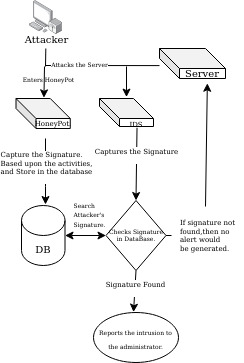
\includegraphics{HIDS}}
\caption{Functionality Diagram}
\label{fig}
\end{figure}

Figure 1 shows that the Honeypot is connected with the same database from which the IDS would be connected to. This provides an easy connectivity between the new signatures generated by the honeypot and the intrustion detection system. The IDS provides a ability to either completely drop the malicious packets or just to generate an alert and send it to the administrator of the system. The honeypot can be made compatible to have a support in which alert generation process uses a high speed redis database, this would help to generate the alert faster. If the IDS is setup to drop the packets then use of a persistent storage like MySQL can also be used.

\subsection{Modules}

The main modules would be:
\begin{itemize}
    

\item  A module to add support for \textit{SSH connectivity}. This would enable the Honeypot to provide a secure shell (SSH) connectivity. A secure-shell functionality is required in the Honeypot so a malicious actor is able to connect to the server/honeypot which would give them the feeling of ``getting an access to real system''. Once the attacker is able to login they can perform various actions like trying to access the data present on the server, trying to escalate the privileges etc. All these actions would be logged by the logger for future analysis.\\

\item A module to add support for \textit{FTP connectivity}. File-Transfer Protocol (FTP) are very common type of protocol used to transfer files from one server to another server. On our honeypot we will provide service which will host a fake/dummy data and will open port 21 i.e FTP service, which can then be used by the attacker to get files out of our honeypot. During this process the attackers activity would be logged. This module would be an important addition to our Honeypot because FTP protocol might give use details like location where the dummy data was transfered to, IP address etc. \\

\item  A module to \textit{generate IDS signature from Honeypot logs}. This module provides the core functionality of this project which is to make more signatures/rules for the IDS which would improve the intrustion detection. Generating specific rules within a predefined and proper format of signature would be important otherwsie SNORT IDS will not use them while operating. For this module we will have to write a parser which will analyze and extract the important information out of the logged data. Once the analysis would end then it will generate the new rules. \\

\item  A module to provide a proper \textit{data synchronization between the IDS and honeypot}. This is required in terms of data management, by having this module we will be easily able to keep a track of all the new signature added by the Honeypot and IDS itself. If we don't add anything to track the data then it is possible to have duplicate data generation which wouldn't be beneficial in any way. \\

\end{itemize}

\section{Timeline}

Because this is written in a very early stage of the project, it is very hard to estimate the workload needed in different parts of the project. Table 1 is only a qualified guess of what amount of time needed in the different stages of the project. We came up with this by calculating the number of Week remaining in our current semester and then decided to split the work according to those weeks.

In the below table the ``W'' represents the Week number.

\begin{table}[htbp]
    \caption{Estimated Timeline}
    \begin{center}
    \begin{tabular}{ | p{3cm} | p{1cm} | p{1cm} | p{3cm} | }
        \hline
            \textbf{Activity} & \textbf{\textit{Start time}} & \textbf{\textit{End time}} & \textbf{\textit{Resources}} \\
        \hline
        Literature Study & W1 & W3 & Web \\
        \hline
        Research Paper & W4 & W12 & Web, articles \\
        \hline
        Implementing Honeypot (module 1) & W6 & W8 & honeynet.org, github.com, articles \\
        \hline 
        Testing module 1 & W9 & W10 & using static code analyzers \\
        \hline
        Updating research paper based on new findings & W10 & W12 & Web, new data gather from honeypot \\
        \hline
    \end{tabular}
    \label{tab1}
    \end{center}
\end{table}


\begin{thebibliography}{00}
\bibitem{b1} Writing Snort Rules | How to write Snort rules and keep your sanity by Martin Roesch
\bibitem{b2} http://books.gigatux.nl/mirror/snortids/0596006616/snortids-CHP-3-SECT-4.html
\bibitem{b3} The honeynet project. http://www.honeynet.org/.
\bibitem{b4} L. Spitzner, e. a.  2004.Know  Your  Enemy  :  Learning  about  SecurityThreats. Addison-Wesley Professional.
\bibitem{b5} Kreibich, C. & Crowcroft, J. 2004. Honeycomb-creating intrusion detection signatures using honeypot.ACM SIGCOMM Computer Communica-tion Review archive, 34(1), 51–56.
\bibitem{b6} Yegneswaran,  V.,  Giffin,  J.  T.,  Barford,  P.,  &  Jha,  S.    2005.An   architecture   for   generating   semantics-aware   signatures.www.cs.wisc.edu/ vinod/nemean.pdf.
\bibitem{b7} Snort. http://www.snort.org/.
\bibitem{b8} A.Sagala, ``Automatic SNORT IDS Rule Generation Based on Honeypot Log,'' Faculty of Informatics & Electrical, Del Institute of Technology,2015
\bibitem{b9} V.Ajaxon,``Building IDS ruess by means of a  honeypot'', NISlab-Norwegian Information Security Laboratory,2005.
\end{thebibliography}
\vspace{12pt}
\end{document}
